\section{Introduction}
\label{sec:intro}
Retrieval-augmented models~\cite{lewis2020rag} struggle when the evidence is spread
across documents that exceed the context window of the reader. Prior work on sparse
transformers~\cite{child2019sparse} reduces the quadratic cost of attention, but does not
address where to look.

We make two contributions. First, we propose a sparse attention prior (Section~\ref{sec:method}).
Second, we evaluate it on three long-context benchmarks (Section~\ref{sec:results}),
see Figure~\ref{fig:overview} for an overview.

\begin{figure}[t]
  \centering
  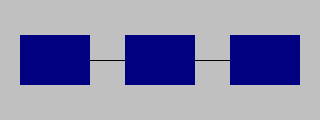
\includegraphics[width=0.8\linewidth]{figures/overview}
  \caption{Overview of the retrieval pipeline with the sparse prior.}
  \label{fig:overview}
\end{figure}
